\chapter{Attentional Networks}
\label{ch:attentional}
To help simplify the learning problem the task was again reframed to improve the signal to noise ratio.
The preprocessing was adjusted such that decay was applied around every event but instead of using the full image only an 11x11 decayed area was kept.
In keeping with previous experiments decay was applied into the past and future to be the input and output. 
Figure \ref{fig:11inoutpair} is an example of such a pair.
%Rather than applying decay to the whole image at uniform time intervals and using that as input the to the network each event was decayed around resulting in many more (albiet similar) training examples.
%However only an 11x11 area around each event was considered meaning the signal to noise ratio was much higher. 

\begin{figure}[h]
    \centering
    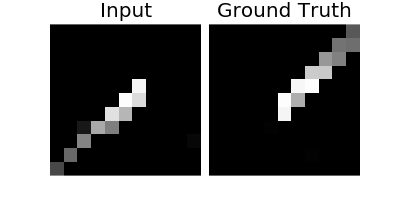
\includegraphics[width=0.5\textwidth]{11xinoutpair_83.png}
    \caption{Example of 11x11 input for an attentional network}
    \label{fig:11inoutpair}
\end{figure}

Figure \ref{fig:11inoutpair} is a cherry picked example of a clean input/output pair though.
The Attentional networks still have a noisy task to solve because every event, including noise, is considered. 
Many of the training examples derived from noise pixels could be filtered out efficiently by demmanding the activity of the example excede some low threshold.
However, the system should be able to deal with noise and setting such a threshold would create another unnecessary hyper-parameter to the model.
Additonally such a parameter would be dependent on the time scale of the data and would need to be adjusted for each task. 
As will be shown the network is able to learn even in the midst of such noise so it is left in. 

%%%%%%%%%%%%%%%%%%%%%%%%%%%%%%      ATTENTIONAL NN    %%%%%%%%%%%%%%%%%%%%%%%%%%%%%%%%%%%%%%
\section{Attentional Directly Connected (ADC) Network}
This network, as the name suggests, is simply a direct connection between the input and output units.
Now that the prediction problem had been broken down into a seemingly simple task it was expected that results could be achieved with a simple network. 
The network details are outlined in table \ref{tb:attnet1def}, with key points being the loss function has returned to the standard S.S.D. instead of the linearly weighted S.S.D. and the number of inputs has drastically decreased. 

\begin{table}[h]
\centering
\begin{tabular}{ | l | l | }
    \hline
    Num. Inputs & 121 \\
    Num. Outputs & 121 \\
    Connectivity & Fully connected \\
    Num. Hidden Layers & 0 \\
    Activation function & Linear, ReLU, Sigmoid \\
    Loss & Sum of Squares Difference \\
    Learning rule & S.G.D. (back propogation) \\
    Learning rate & 0.1 \\
    Mini-batch size & 100 \\
    \hline
\end{tabular}
\caption{Features of the Attentional Directly Connected Networks}
\label{tb:attnet1def}
\end{table}

\subsection{Linear activation}
The simplest ADC network considered had only a linear activation to compute outputs. 
This proved to be enough for the network to learn to make coherent predictions. 
The two datasets (8 Angle and Arbitrary Angle) were considered, a network was trained on each and then made predictions on a set of validation data from it's own dataset and other dataset to see how it could generalise.

\subsubsection{Trained on 8 Angle}

\begin{figure}
    \centering
    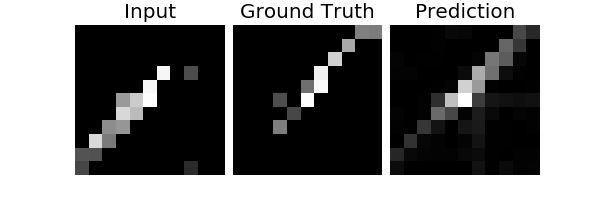
\includegraphics[width=0.8\textwidth]{ADC_8a_8a_13.png}
    \caption{A good prediction from ADC trained on 8A and predicting 8A.}
    \label{fig:ADC_8a_8a_crct} 
\end{figure}

\begin{figure}
    \centering
    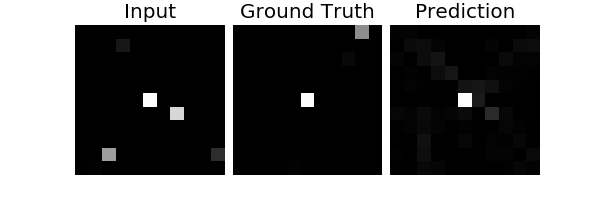
\includegraphics[width=0.8\textwidth]{ADC_8a_8a_7.png}
    \caption{The ADC network with a noisy input}
    \label{fig:ADC_8a_8a_noisy}
\end{figure}

Figures \ref{fig:ADC_8a_8a_crct} and \ref{fig:ADC_8a_8a_noisy} show how the linearly activated ADC network trained on the 8 Angle dataset predicted in two cases from the 8 Angle validation set.
% TODO Make this an even more correct image and use this particular img (13) later to discuss problems
In figure \ref{fig:ADC_8a_8a_crct} the network is performing well and gives a prediction which is quite similar the ground truth (ignoring noise). 
Figure \ref{fig:ADC_8a_8a_noisy} is a noisy training example.
The label does not intuitively follow from the input and the network only outputs small values.
However the network does predict faintly along the top left diagonal which is sensible when considering the input has two pixels along the bottom right diagonal (the closer of which is highty active making it resemble a decayed path). 
%However the network has noticed two pixels active along the bottom right diagonal (one of which is highly active) and the network predicts a faint output along the top left diagonal.

\begin{figure}
    \centering
    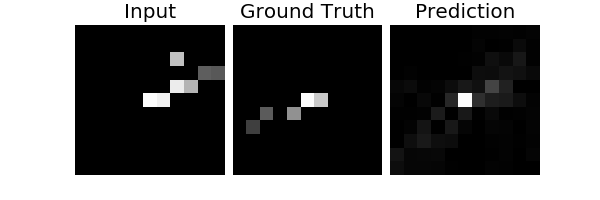
\includegraphics[width=0.8\textwidth]{ADC_8a_aa_4.png}
    \caption{ADC network trained on 8 angles struggles to predict inbetween paths}
    \label{fig:ADC_8aNoaa}
\end{figure}

\begin{figure}
    \centering
    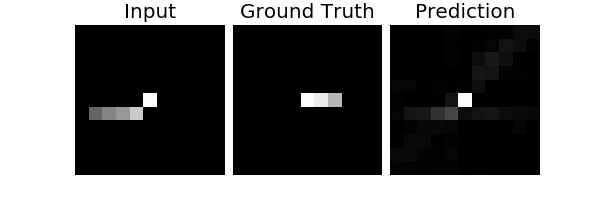
\includegraphics[width=0.8\textwidth]{ADC_8a_aa_46.png}
    \caption{ADC network predicting a slight off angle input}
    \label{fig:ADC_8aNoaa_fork}
\end{figure}

The network performing well on its own validation set is a success in itself but raises the question of how it will generalise from 8 Angles to arbitrary angles.
It was hypothesised the network might be able to use a combination of known angles to represent the new angles in the Arbitrary Angle dataset.
This was not the case though, figure \ref{fig:ADC_8aNoaa} shows the network stuggling to predict the motion.
Most of the activity in the prediction falls in the East North-East section which is where the input was.
There is some very limited activity that matches the label but this is insignificant compared to previous predictions. 
Further figure \ref{fig:ADC_8aNoaa_fork} shows a slightly off center input which looks similar to an angle from the 8 Angle Dataset. 
The network has trouble interpreting this and make 3 faint predictions being the top right diagonal, to the right edge and along the input.
This suggests the network is not able to efficiently represent the arbitrary angles as some combination of the 8 angles it learnt and could perform reasonably well.

An additional interesting case which further supports this claim is seen in figure \ref{fig:ADC_8aNoaa_special} which shows the network suffering from some neatly aligned noise. 
The network is well equipped to deal with inputs coming from one angle at a time but this noise makes it appear as if two dots may be crossing paths. 
The networks behaviour to predict two strong output paths shows that each input path (and its predictions) are happening independently of any the rest of the input.
If the network was representing the input as an angle it would be reasonable to expect that the prediction might be a blur in the top right corner of the prediction.  
Instead this clear prediction of two paths suggests the network is simply learning to map between areas of the input to the output. 

\begin{figure}
    \centering
    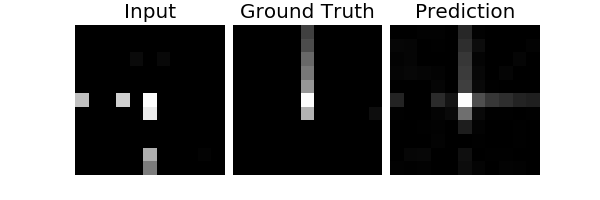
\includegraphics[width=0.8\textwidth]{ADC_8a_aa_15.png}
    \caption{ADC network predicting two paths due to noise}
    \label{fig:ADC_8aNoaa_special}
\end{figure}


\subsubsection{Trained on Arbitrary Angle}
It follows that a network trained on only 8 Angles might have trouble generalising to arbitrary angles so a second network was trained on the arbitrary angles dataset. 
In general the network trained on Arbitrary Angle data was less confident in its predictions (magnitude of predictions were lower) but it had a wider area of guessing. 
This is illustrated in figure \ref{fig:ADC_aaaa_crct} in where the prediction has many faintly coloured squares, in contrast to the more confident predictions made in figure \ref{fig:ADC_8a_8a_crct} by the network trained on the 8 Angle data.

\begin{figure}[h]
    \centering
    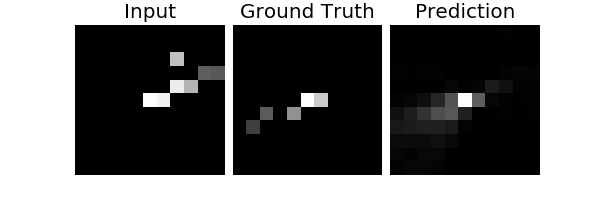
\includegraphics[width=0.8\textwidth]{ADC_aa_aa_4.png}
    \caption{ADC network trained on Arbitrary Angle data correctly predicting}
    \label{fig:ADC_aaaa_crct}
\end{figure}



\begin{figure}[h]
    \centering
    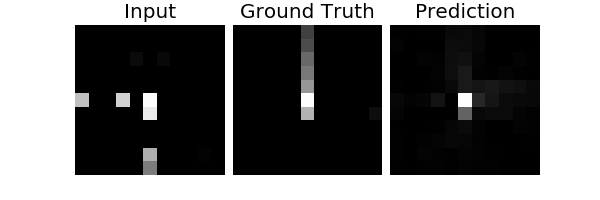
\includegraphics[width=0.8\textwidth]{ADC_aa_aa_15.png}
    \caption{ADC network trained on Arbitrary Angle data predicting two paths due to noise}
    \label{fig:ADC_aaaa_twopath}
\end{figure}

\begin{figure}[h]
    \centering
    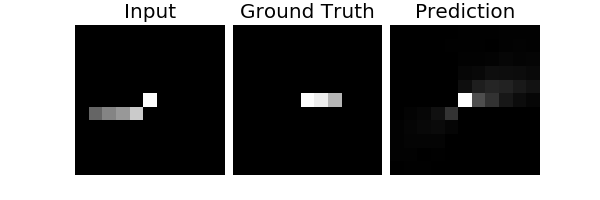
\includegraphics[width=0.8\textwidth]{ADC_aa_aa_46.png}
    \caption{ADC network trained on Arbitrary Angle data predicting a slight off angle input}
    \label{fig:ADC_aaaa_fork}
\end{figure}




%%%%%%%%%%%%%%%%%%%%%%%%%%%%%%      ATTENTIONAL NN    %%%%%%%%%%%%%%%%%%%%%%%%%%%%%%%%%%%%%%
\section{Attentional Hidden Layer (AHL) Network}

Discuss results of using a hidden layer and the improvements if any


%%%%%%%%%%%%%%%%%%%%%%%%%%%%%%      AUTO ENCODE     %%%%%%%%%%%%%%%%%%%%%%%%%%%%%%%%%%%%%%
\section{Auto Encoder}
How much could be cleaned up
Retry other networks with cleaned up data.

